\
% csp.tex — The Cosmic Seal Protocol (arXiv-ready single-file source)
\documentclass[11pt]{article}

\usepackage[a4paper,margin=1in]{geometry}
\usepackage{newtxtext,newtxmath} % modern replacement for 'times'
\usepackage{hyperref}
\usepackage{graphicx}
\usepackage{authblk}
\usepackage{microtype}
\usepackage{enumitem}

\hypersetup{
  colorlinks=true,
  urlcolor=black,
  linkcolor=black,
  citecolor=black,
  pdftitle={The Cosmic Seal Protocol},
  pdfauthor={Matthew LaBarre},
  pdfkeywords={cryptographic provenance, relativity, ephemeris, decentralization, accountability}
}

\title{The Cosmic Seal Protocol\\
Relativistic Cryptographic Provenance through Celestial Motion}

\author[ ]{Matthew LaBarre}
\affil[ ]{Independent Researcher and Steward (Anchor Point)}
\affil[ ]{\texttt{csp@cbarl.org}}
\date{September 08, 2025} %% printed date

\begin{document}
\maketitle

\begin{abstract}
We present the \emph{Cosmic Seal Protocol} (CSP), a cryptographic method for provenance that binds digital artifacts to spacetime intervals. CSP leverages continuous celestial motion as a public witness. Instead of static timestamps or institutional authorities, CSP encodes a two-timestamp window $(t_{\text{in}}, t_{\text{out}})$ and, depending on variant, a frame anchor (physical or logical location) and/or a compact celestial baseline. Two interoperable variants are defined. \textbf{CSL-Min} records times, a monotonic duration, and an optional physical or logical location; verifiers independently recompute celestial states from public ephemerides (e.g., VSOP87 or JPL DE440) to test plausibility. \textbf{CSL-Plus} adds a \emph{COSMIC\_BASE} (RA/Dec tuples for Sun$\rightarrow$Saturn at $t_{\text{in}}$) and $\Delta t=t_{\text{out}}-t_{\text{in}}$, enabling deterministic re-derivation of the sky at both endpoints. Seals are computed over canonical JSON (RFC 8785) with standard hashes (e.g., SHA-384), yielding \emph{relativistic fingerprints}. We analyze trust and threat models (clock and ephemeris manipulation, location spoofing, replay) and show how independent recomputation provides strong public verifiability without heavy infrastructure. A conversational prototype, \emph{Chat Seal}, demonstrates interactive sealing with negligible overhead. CSP is released under open, stewardship-oriented licenses to prioritize accessibility and public benefit.
\end{abstract}
\begin{figure}[t]
  \centering
  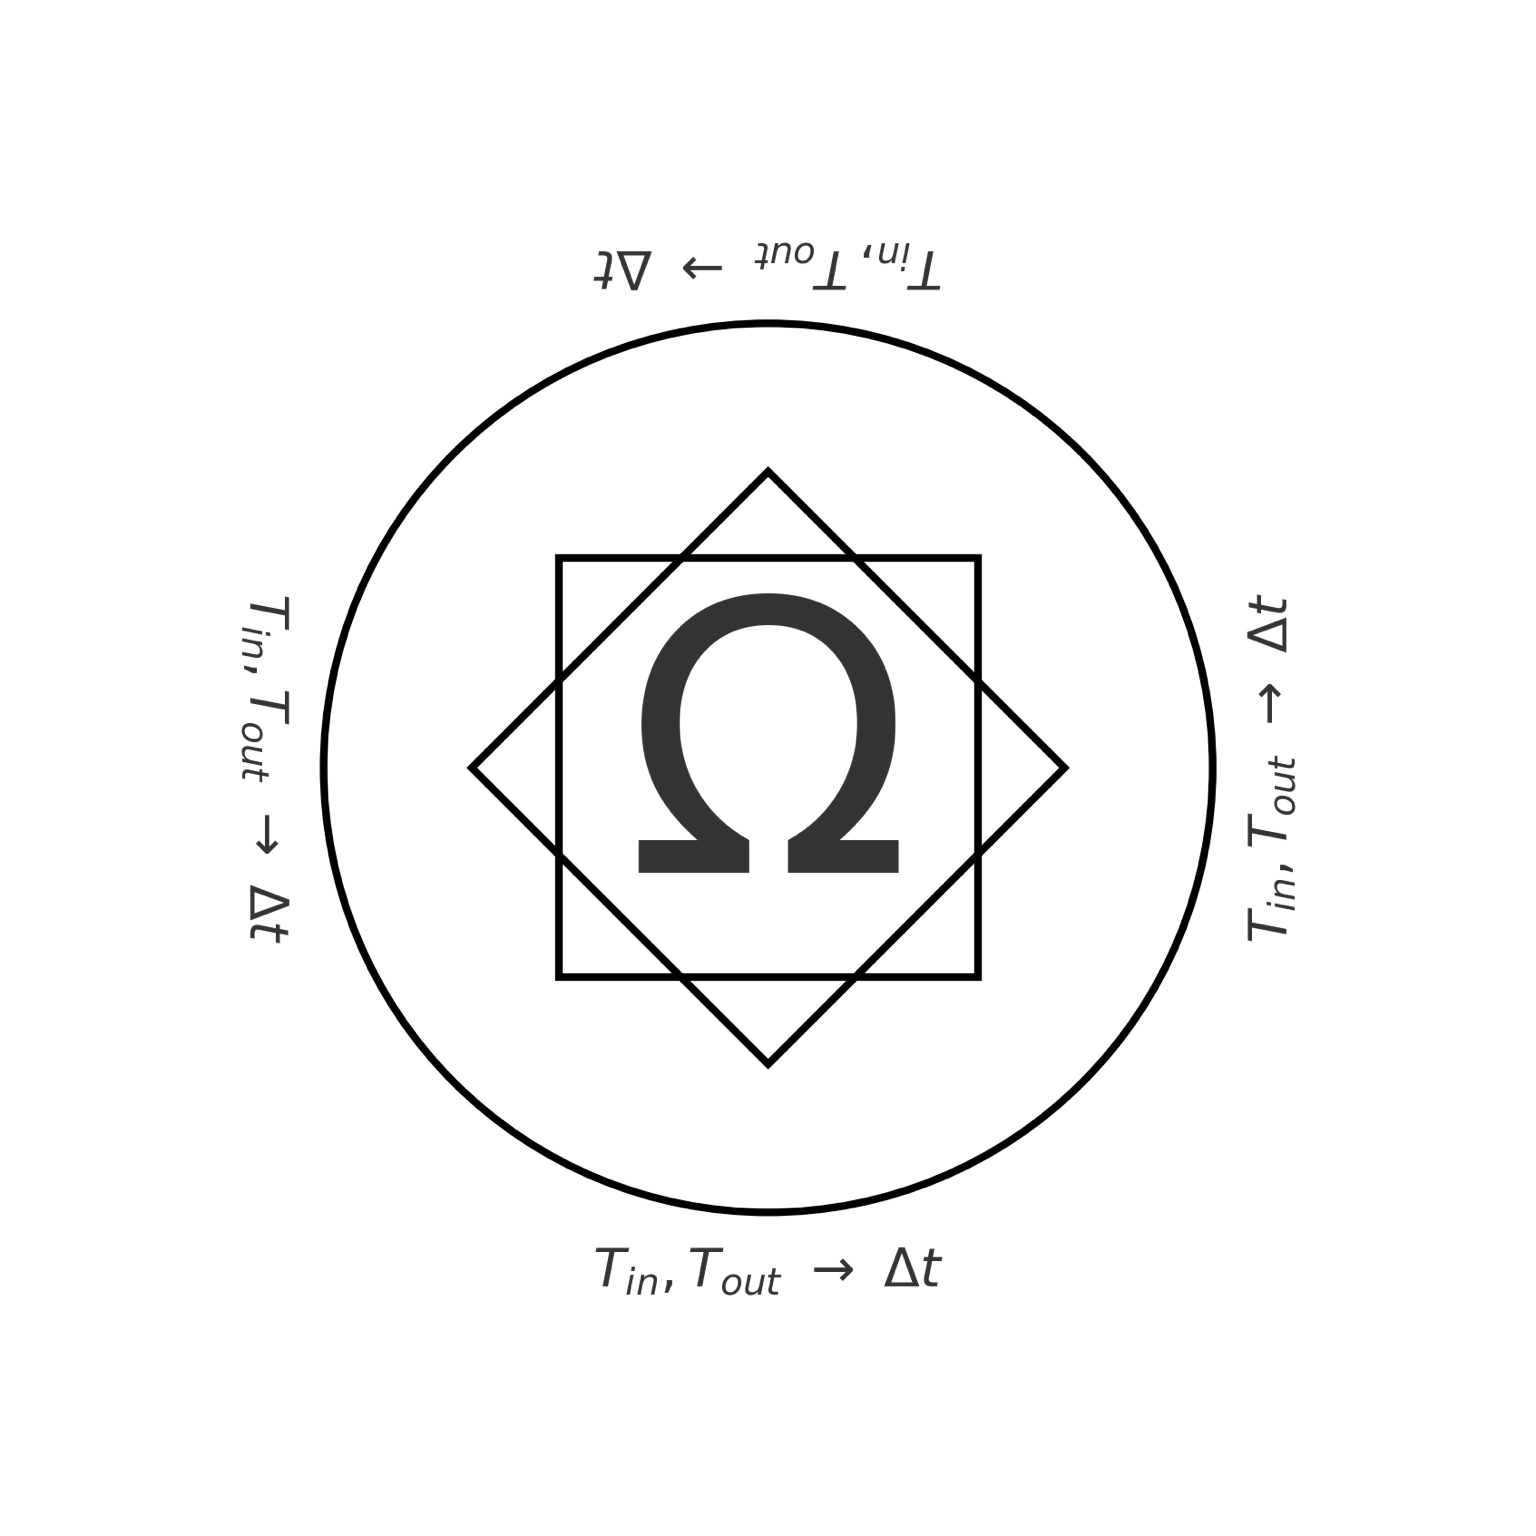
\includegraphics[width=0.45\linewidth]{rahuyantra_omega_outward.png}\hfill
  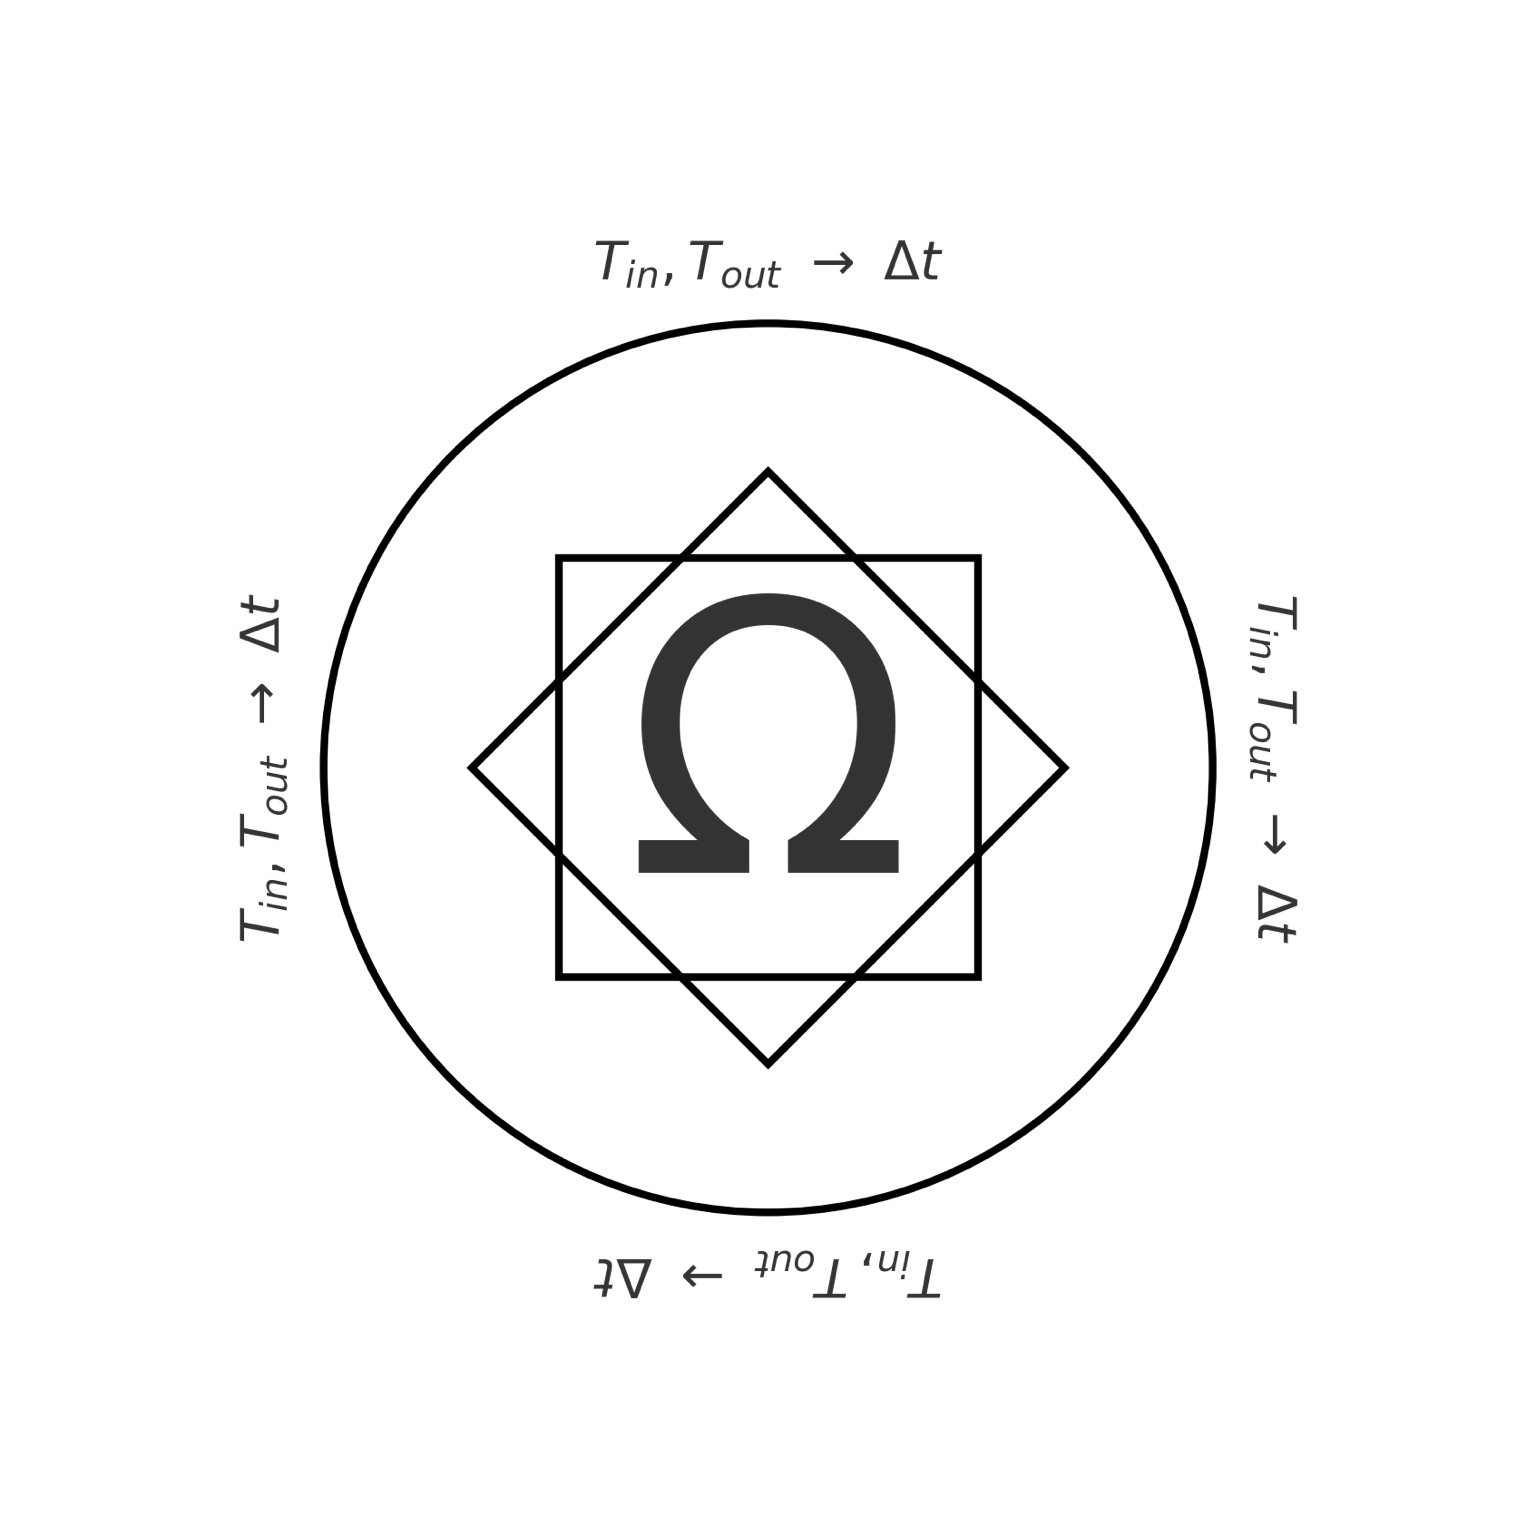
\includegraphics[width=0.45\linewidth]{rahuyantra_omega_inward.png}
  \caption{Cosmic Seal variants (open request, left; sealed return, right). Two overlapping squares (octagram) within a circle, with central $\Omega$ and the etched interval formula $T_{in}, T_{out} \to \Delta t$ oriented outward (request) or inward (return).}
  \label{fig:csp-variants}
\end{figure}


\vspace{0.3em}
\noindent\textbf{Keywords:} cryptographic provenance; relativity; \emph{panta rhei}; ephemerides; decentralization; accountability.

\section{Introduction}
Digital societies increasingly depend on the ability to attest: to say ``this was made here, then, by this process,'' and to make that claim stand up outside the system that issued it. Conventional approaches lean on centralized authorities (certificate hierarchies) or global consensus machinery (blockchains). Both succeed in many settings; both also center \emph{static} assertions---single timestamps, named identities, global ledgers---that can be brittle or costly when what is needed is a small, portable, independently checkable proof.

This work began from a practical need for autonomy and verifiable truth in legal--digital workflows. The immediate problem was mundane: seal a chat message or micro-artifact in a way that survives platform boundaries and institutional churn, without forcing participants to register with a CA or anchor to an energy-intensive chain. That pragmatic constraint led to a broader critique of centralized trust models and to a simple observation from physics and philosophy: in Einsteinian relativity there is no absolute frame; in Heraclitean terms, \emph{panta rhei}---everything flows. The sky's continuous motion provides a public, recomputable witness.

We formalize two variants: \textbf{CSL-Min} and \textbf{CSL-Plus}. Both bind an artifact to a spacetime interval and a frame anchor. Verification requires no registry: only the artifact bytes, seal JSON, and access to public ephemerides. We present the protocol, analyze its security, discuss deployment, and position it against timestamp authorities, PKI, and blockchains.

\subsection*{Contributions}
\begin{itemize}[leftmargin=1.2em]
\item Reframe provenance around relativistic fingerprints based on spacetime deltas and celestial dynamics.
\item Design clear object schemas, canonicalization rules, and hash constructions for \emph{CSL-Min} and \emph{CSL-Plus}.
\item Analyze adversary model and practical mitigations (clock skew, location spoofing, ephemeris choice, replay).
\item Implement a conversational prototype (\emph{Chat Seal}); provide guidance for ephemeris selection and serialization pitfalls; release under licenses prioritizing stewardship and public use.
\end{itemize}

\section{Theoretical Foundations}
Heraclitus stressed that one cannot step into the same river twice; change is constitutive of identity, not a defect. Applied to information systems, provenance should be anchored to \emph{intervals of motion}. Einstein's relativity dismantles absolute simultaneity; digital timekeeping that assumes a universal clock bakes in fragile metaphysics. CSP accepts relativity as a constraint and leverages the sky as a public witness. Ephemerides such as VSOP87 and JPL DE440 are open and widely implemented; anyone can recompute positions and check consistency.

\section{Protocol Design}
All objects are encoded as canonical JSON (RFC 8785). The artifact record (\texttt{RPP}) includes the artifact name, optional base64 bytes, a mandatory SHA-384 digest, issuance time, and optional context. The \texttt{CSL} record stores $t_{\text{in}}$, $t_{\text{out}}$, a monotonic duration, a location object (physical and/or logical anchors), the variant, and minimal session metadata.

Two hashes are produced: \(S1 = H(J(RPP)\parallel H(P))\) tying the artifact to its digest; and \(S2\) tying the seal record to the artifact digest. For \textbf{CSL-Min}, \(S2_{\text{lite}} = H(J(\{t_{\text{in}},t_{\text{out}},duration_{mono},location\})\parallel H(P))\). For \textbf{CSL-Plus}, \(S2_{\text{full}} = H(H(J(COSMIC\_BASE))\parallel J(\{t_{\text{in}},t_{\text{out}}\})\parallel H(P))\), where \texttt{COSMIC\_BASE} contains RA/Dec for Sun, Moon, Mercury--Saturn at \(t_{\text{in}}\).

\paragraph{Verification.} Recompute the artifact digest; recompute celestial states at $t_{\text{in}}$ (and $t_{\text{out}}$ if used) to check consistency with the published location and/or \texttt{COSMIC\_BASE}; reconstruct \(S1\) and \(S2\) from canonical JSON; compare to the published values.

\section{Security Analysis}
\subsection*{Adversary Model and Properties}
We assume an attacker who controls the channel, can tamper with local clocks and location metadata, and has substantial compute short of breaking SHA-384. CSP provides artifact and seal integrity, replay resistance, frame-consistency via ephemeris recomputation, and privacy-preserving minimality (logical location anchors and redaction are supported).

\subsection*{Threat Scenarios and Mitigations}
Clock tampering is constrained by a monotonic duration; location spoofing is tempered by verifiers' ability to reject unverifiable anchors; ephemeris manipulation is mitigated by independent recomputation (VSOP87, DE440); substitution and replay fail because digests bind artifacts to intervals; cryptographic obsolescence is addressed by hash agility.

\section{Implementation Considerations}
\paragraph{Reference Prototype.} \emph{Chat Seal} records $t_{\text{in}}$ on command and $t_{\text{out}}$ on completion; even short intervals yield nonzero celestial motion.

\paragraph{Ephemerides.} VSOP87 offers compact analytic series suitable for low-power devices; JPL DE440 provides higher precision at higher resource cost. Implementations should record which model was used.

\paragraph{Resource Footprint.} CSL-Min seals are a few hundred bytes; CSL-Plus adds $\sim$KB for \texttt{COSMIC\_BASE}. Compute cost is milliseconds on commodity hardware. No global ledger is maintained.

\paragraph{Standards.} RFC 8785 (JSON canonicalization) and RFC 3339 (timestamps) ensure interoperability. CSP is hash-agnostic but defaults to SHA-384 (FIPS 180-4).

\section{Related Work}
Trusted timestamping (RFC 3161) relies on a timestamp authority; PKI (RFC 5280) binds names to keys via certificate authorities; blockchains provide decentralized ordering at the cost of heavy consensus. CSP differs by grounding provenance in recomputable physics with self-contained seals. Physics-based beacons (e.g., NIST) distribute measurements via authorities; CSP requires no broadcast source.

\section{Conclusion}
By recognizing the sky as an inexhaustible, recomputable witness, CSP reframes provenance around intervals and motion rather than static instants or institutional fiat. Lightweight, accessible, and physically grounded, CSP offers a practical tool for cryptographic provenance that anyone can verify. Future work includes higher-precision seals, cross-ephemeris verification, and integrations that join CSP's \emph{when/where} with signature systems' \emph{who}.

\begin{figure}[t]
  \centering
  % Place your compass/star graphic file in the same directory and name it accordingly:
  \includegraphics[width=0.6\linewidth]{compass_star.jpg}
  \caption{Cosmic Seal emblem (conceptual): the \emph{anchor point} at center and an eight-point star tracing motion around a relational frame.}
  \label{fig:emblem}
\end{figure}

\section*{Stewardship \& Licensing}
The specification and paper are licensed under \textbf{CC BY-NC 4.0} (attribution, noncommercial). Reference implementations are licensed under \textbf{AGPLv3}. This pairing keeps CSP accessible for research and public use while preventing enclosure. The author serves as the \emph{anchor point} (steward) for the canonical specification and reference implementation.

\vspace{0.5em}
\noindent\textbf{Author Positionality.} This work is contributed in an independent capacity; the neurodivergent vantage that motivated it---skeptical of defaults, biased toward first principles---was essential in noticing that everyday physics can shoulder part of our provenance burden.

\begin{thebibliography}{12}

\bibitem{einstein1905} A.~Einstein, ``Zur Elektrodynamik bewegter K\"orper,'' \emph{Annalen der Physik}, vol.~17, pp.~891--921, 1905. (English: \emph{On the Electrodynamics of Moving Bodies}.)

\bibitem{einstein1916} A.~Einstein, ``Die Grundlage der allgemeinen Relativit\"atstheorie,'' \emph{Annalen der Physik}, vol.~49, pp.~769--822, 1916. (English: \emph{The Foundation of the General Theory of Relativity}.)

\bibitem{heraclitus} Heraclitus, \emph{Die Fragmente der Vorsokratiker}, eds. H.~Diels and W.~Kranz, 6th~ed., Weidmann, 1952. (Fragments DK22B12, DK22B49a.)

\bibitem{rfc8785} J.~Br{\"u}nink and K.~Zyp, ``JSON Canonicalization Scheme (JCS),'' RFC~8785, IETF, 2020. \url{https://datatracker.ietf.org/doc/html/rfc8785}.

\bibitem{rfc3339} G.~Klyne and C.~Newman, ``Date and Time on the Internet: Timestamps,'' RFC~3339, IETF, 2002. \url{https://datatracker.ietf.org/doc/html/rfc3339}.

\bibitem{rfc5280} D.~Cooper, S.~Santesson, S.~Farrell, S.~Boeyen, R.~Housley, and W.~Polk, ``Internet X.509 Public Key Infrastructure Certificate and CRL Profile,'' RFC~5280, IETF, 2008.

\bibitem{rfc3161} C.~Adams, P.~Cain, D.~Pinkas, and R.~Zuccherato, ``Internet X.509 Public Key Infrastructure Time-Stamp Protocol (TSP),'' RFC~3161, IETF, 2001.

\bibitem{fips180-4} NIST, ``FIPS PUB 180-4: Secure Hash Standard (SHS),'' U.S. Department of Commerce, 2015. doi:10.6028/NIST.FIPS.180-4.

\bibitem{bretagnon1988} P.~Bretagnon and G.~Francou, ``Planetary Theories in Rectangular and Spherical Variables: VSOP87 Solutions,'' \emph{Astronomy and Astrophysics}, vol.~202, pp.~309--315, 1988.

\bibitem{park2021} R.~S.~Park, W.~M.~Folkner, R.~A.~Jacobson, and J.~G.~Williams, ``The JPL Planetary and Lunar Ephemerides DE440 and DE441,'' \emph{The Astronomical Journal}, 161(3):105, 2021. doi:10.3847/1538-3881/abd414.

\bibitem{nakamoto2008} S.~Nakamoto, ``Bitcoin: A Peer-to-Peer Electronic Cash System,'' 2008. \url{https://bitcoin.org/bitcoin.pdf}.

\bibitem{nistbeacon} NIST, ``NIST Randomness Beacon,'' 2011. \url{https://beacon.nist.gov/home}.
\end{thebibliography}

\end{document}


\section*{Author Statement \& Seal}
Signed on September 08, 2025 by \textbf{MATTHEW RUSSELL LABARRE} (steward/anchor). The author affirms that this submission reflects the canonical CSP specification as of the date above. A cryptographic seal accompanies the source bundle.

\noindent\textbf{CSP BangCheck (source artifacts, SHA-384):}
\begin{verbatim}
!BEGIN BANGCHECK
csp.tex · SHA-384=0273bdb808867e5f7ddb3dff36738efcf390c6cb76dd59d9f55d3390bac2e68d7fd476f49fbbce4f621939e522ccfc7a
rahuyantra_omega_outward.png · SHA-384=2b3f32fe52981172eec1f05705257c28295870d5d017aeb01bb62f61ab9b7ac71fb5d0013487576e3113c2b0d96a49f5
rahuyantra_omega_inward.png · SHA-384=94c870ab5c57c969903521fa45b59b777d4b53d12ecfb5c8ea212bd560c84cc932b5fc1a11e55cdfc7ef25f3b0ea4ec9
rahuyantra_omega_outward.svg · SHA-384=a2d9beab96357d84d142dec13480e764d3771486d11e439557ac9bbd1c2281c554ea005bb71ab6399deaf153cd1e298a
rahuyantra_omega_inward.svg · SHA-384=911593d279f610ec696694f6b6c8a80405fe0791e7de0c91da43f38392469bcf7e15695d286ad1de60a061a6cfe57378
compass_star.png · SHA-384=ea803a1b42a45c62d72bf3152a33e2d5460c6572bdce8bcd2a57c5940261216f6169cc0fe1e96c27788efbceae3c86b9
compass_star.jpg · SHA-384=bb40556ed2c0a20cae10fc6890dbb614c03a339f4d7c3f96f18b6a79c25b40d646bfab592d41055a0113add968152db6
!END BANGCHECK
\end{verbatim}

\noindent\emph{Note:} After arXiv compilation, the final PDF's digest can be computed and appended to the ledger to complete the CSL record.

